\section{A Characterization Study on the First Run~\label{sec:sodb9_r3_hist}} 
This section further discusses the first run of 
INC with its task length increasing from 1 second to 4096 seconds via EMPv5 with no Step 2. 
The detailed description of the base data is from Table~\ref{tab:exp_notes1}.

\subsection{Summary of Histograms}

\begin{figure}[hp!]
\vspace{-.3in}
	\centering
	\includegraphics[scale=0.5,angle=270]{u_s_time/3d_plot.eps}\label{fig:3d_plot}
	\caption{3D histograms on INC~\label{fig:hist3d}}
\end{figure}

\subsection{Absolute and Relative Variance over Increasing Task Length}

\begin{figure}[hp!]
	\centering
	\subfigure[Standard deviation (absolute)]{
		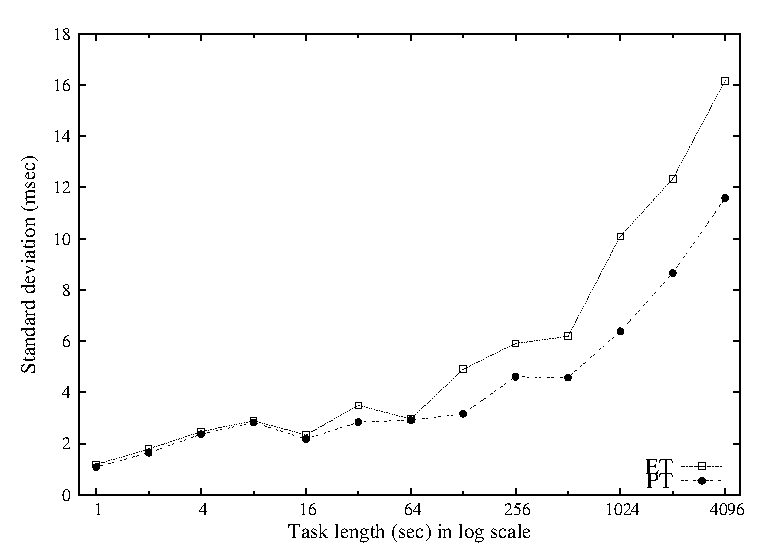
\includegraphics[scale=0.6]{u_s_time/overall_std.eps}
		\label{fig:overall_std}
	}
	\subfigure[Coefficient of variation (relative)]{
		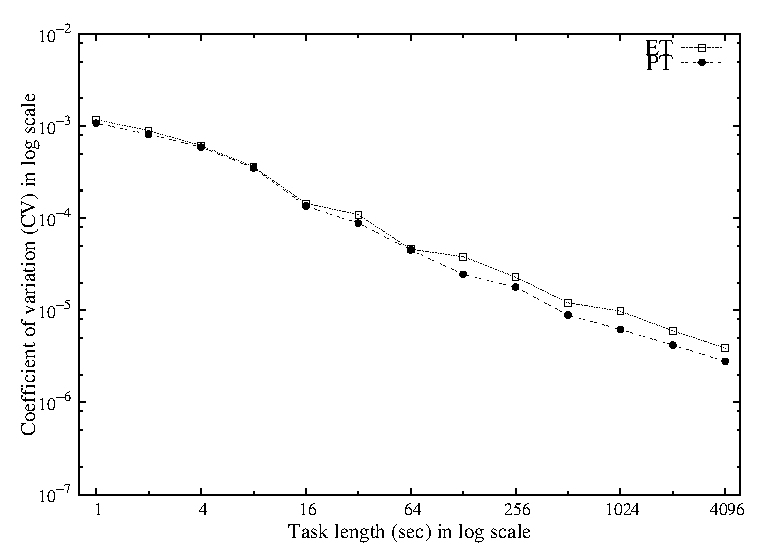
\includegraphics[scale=0.6]{u_s_time/overall_re.eps}
		\label{fig:overall_re}
	}
	\caption{Absolute and relative variances~\label{fig:cv_inc}}
\end{figure}

\pagebreak
\newpage